\documentclass[problem]{mcs}

\begin{pcomments}
  \pcomment{FP_seating_around_a_round_table}
  \pcomment{by Megumi F09}
\end{pcomments}

\pkeywords{
  combinatorics
  permutation
  division rule
  inclusion-exclusion
}

%%%%%%%%%%%%%%%%%%%%%%%%%%%%%%%%%%%%%%%%%%%%%%%%%%%%%%%%%%%%%%%%%%%%%
% Problem starts here
%%%%%%%%%%%%%%%%%%%%%%%%%%%%%%%%%%%%%%%%%%%%%%%%%%%%%%%%%%%%%%%%%%%%%

\begin{problem}
  \bparts The queen and king of hearts decide to host a poker game and
  invite their best friends: the queens and kings of clubs, diamonds, and
  spades.  The queen has a round table that can seat exactly $8$ people
  for the guests (the $3$ other couples) and the host and hostess (her
  husband and herself).

\ppart \mbox{}
\begin{center}
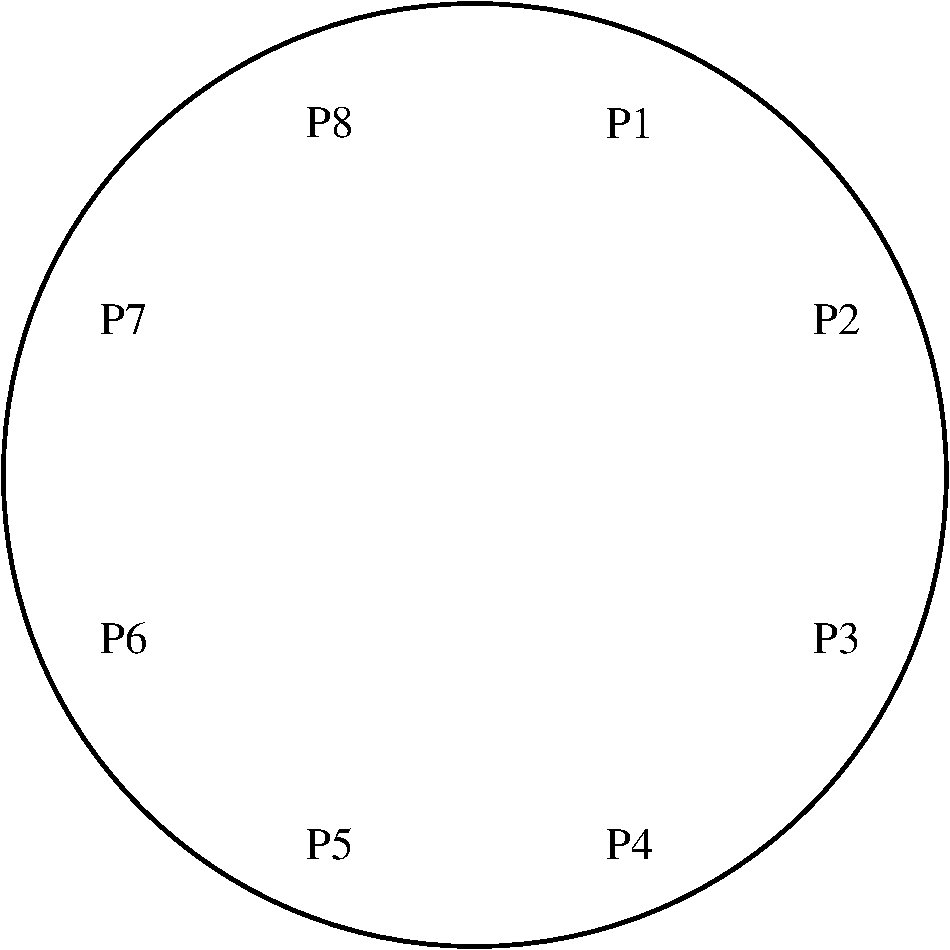
\includegraphics[height=1.5in]{figures/round_table.pdf}
\end{center}

If each of the chairs around the table is marked with a distinct symbol in
$\set{P_1, P_2, \ldots, P_8}$, how many ways can the queen seat the $8$
people in the $8$ chairs?

\examspace[1.5in]
\begin{solution}
$8!$
\end{solution}

\ppart 
\newcommand{\spa}{\spadesuit}
\newcommand{\hea}{\heartsuit}
\newcommand{\dia}{\diamondsuit}
\newcommand{\clu}{\clubsuit}

%\begin{definition}

Two {\bf seatings} are defined to be equivalent, if one can be obtain the
other though a rotation.  For example, the two seatings below are
considered equivalent:

\begin{center}
\begin{tabular}{|l|l|l|l|l|l|l|l|}
\hline
$P_1$ & $P_2$ &$P_3$ &$P_4$ & $P_5$ & $P_6$ & $P_7$ & $P_8$ \\ \hline \hline
$K\spa$ & $Q\spa$ & $K\hea$ & $Q\hea$ & $K\dia$ & $Q\dia$ & $K\clu$ & $Q\clu$ \\ \hline
$K\dia$ & $Q\dia$ & $K\clu$ & $Q\clu$ & $K\spa$ & $Q\spa $ & $K\hea$ & $Q\hea$ \\ \hline 
\end{tabular}
\end{center}

%\begin{eqnarray*}
%K\spa, Q\spa, K\hea, Q\hea, K\dia, Q\dia, K\clu, Q\clu \\
%Q\hea, K\dia, Q\dia, K\clu, Q\clu, K\spa, Q\spa, K\hea 
%\end{eqnarray*}
%\end{definition}

How many distinct \textbf{seatings} are there?

\examspace[1in]
\begin{solution}
$\frac{8!}{8} = 7!$
\end{solution}

%\inhandout{\instatements{\newpage}}

\ppart How many distinct {\bf seatings} are there if the queen and king of
hearts must be seated next to each other?
{\em Hint:~Think of the king and queen as a single unit.}

\examspace[2in]
\begin{solution}
$2! \cdot \frac{7!}{7} = 2 \cdot 6!$
\end{solution}

\ppart How many distinct \textbf{seatings} are there if the queen and king
of hearts must be seated next to each other, and the queen and king of
spades must be seated next to each other?

\examspace[2in]
\begin{solution}
$2! \cdot 2! \cdot \frac{6!}{6} = 4 \cdot 5!$
\end{solution}

\ppart
How many distinct {\bf seatings} are there where no one is seated next to their spouse?
{\em Hint:~Use inclusion-exclusion.} 

\examspace[2in]
\begin{solution}
\begin{eqnarray*}
\mbox{Answer} &=& \{\mbox{Total seatings}\} \\
&-& {4 \choose 1} \times \{\mbox{Seatings with at least one couple seated together}\} \\
&+& {4 \choose 2} \times \{\mbox{Seatings with at least two couples seated together}\} \\
&-& {4 \choose 3} \times \{\mbox{Seatings with at least three couples seated together}\} \\
&+& {4 \choose 4} \times\{\mbox{Seatings with the four couples seated together}\} \\
&=& 7! - 4 \cdot (2 \cdot 6!) + 6 \cdot (4\cdot 5!) - 4 \cdot (8 \cdot 4!) + 1 \cdot (16 \cdot 3!)
\end{eqnarray*}
\end{solution}

\eparts
\end{problem}

%%%%%%%%%%%%%%%%%%%%%%%%%%%%%%%%%%%%%%%%%%%%%%%%%%%%%%%%%%%%%%%%%%%%%
% Problem ends here
%%%%%%%%%%%%%%%%%%%%%%%%%%%%%%%%%%%%%%%%%%%%%%%%%%%%%%%%%%%%%%%%%%%%%

\endinput
